\documentclass[12pt]{report}
\title{Mid Term Project}
\usepackage{amsmath}
%\usepackage{maplestd2e}
\usepackage{tikz}
\usetikzlibrary{arrows.meta,shapes.misc,patterns,shapes.symbols,decorations.pathreplacing,decorations}
\usepackage{amssymb}
\AtBeginDocument{\renewcommand{\chaptername}{}}
\usepackage{microtype}
\usepackage[bottom=30 mm, top=25 mm, left=25 mm, right=25 mm]{geometry}
\usepackage{multicol}
\usepackage{titlesec} 
\usepackage{graphicx}
\usepackage{listings}
\usepackage{xcolor}
\usepackage{amsmath}
\usepackage{subfigure}
\usepackage{subfig}
\usepackage{wasysym}
\usepackage{mathtools}
\usepackage{wrapfig}
\usepackage{float}
\usepackage{lipsum} 
%\usepackage[framed,numbered,autolinebreaks,useliterate]{mcode}
\lstset{
    breaklines=true,
    tabsize=3,
    showstringspaces=false
}

\lstdefinestyle{Common}
{
    extendedchars=\true,
    language={[Visual]Basic},
    frame=single,
    framesep=3pt,
    framerule=0.4pt,
    xleftmargin=3.4pt,
    xrightmargin=3.4pt,
    rulecolor=\color{red}
}

\lstdefinestyle{A}
{
    style=Common,
    backgroundcolor=\color{yellow!10},
    basicstyle=\scriptsize\color{black}\ttfamily,
    keywordstyle=\color{black},
    identifierstyle=\color{black},
    stringstyle=\color{red},
    commentstyle=\color{black}
}

\makeatletter 
\renewcommand\chapter{\thispagestyle{plain}%
\global\@topnum\z@
\@afterindentfalse
\secdef\@chapter\@schapter}
\makeatother 

\titleformat{\chapter}{\bfseries\Huge}{\thechapter.\quad}{0em}{}


\usepackage[utf8]{inputenc}
\parindent0pt

\begin{document}

%\setlength{\parindent}{3ex} 

\begin{large}

\thispagestyle{empty}
\begin{center}
\begin{figure}[t]
\centering
%
\includegraphics[scale=0.52]{sdsu_logo.png}
\end{figure}
\end{center}
\begin{center}
\Large{Department of Mathematics and Statistics}
\end{center}
\begin{center}
\Large{Prof. Joseph Mahaffy}
\end{center}
\begin{center}
\Large{Math 636, Mathematical Modeling}
\end{center}
\begin{verbatim}



\end{verbatim}
\begin{center}
\textbf{\Huge{Homework Assignment}}
\end{center}
\begin{verbatim}


\end{verbatim}
\rule{16,5 cm}{0.4pt}\\
\begin{center}
\textbf{\LARGE{Models with delay}}\\[0,7 cm]
\end{center}
\rule{16,5 cm}{0.4pt}
\begin{verbatim}


\end{verbatim}

\begin{center}
 \textbf{by Matteo Polimeno} \\ 
\textbf{12/14/2017}\\

\end{center}
\end{large}


\newpage

%\tableofcontents
\newpage

\sloppy

\newpage


\chapter{Problem 1}
\section{Part a}
Genetic repression is one of the mechanisms that controls genetic expression in bacteria. A classic example is given by a dimeric protein called Tryptophane-repressor, found and studied in the \textit{E. Coli}. Repressors are, in general, DNA or RNA-binding proteins whose job is to inhibit the expression of one or more genes by binding to the associated operator. \\
As for the Tryptophane repressor, this protein controls the \textit{E. Coli} aminoacids' metabolism through a varieties of processes. For instance, if the aminoacid Tryptophan is not found in the cell, then the repressor is inactive and the enzyme Tryptophane-synthase is produced, and, since synthases are enzymes that synthetize chemical species, naturally the concentration of the tryptophan in the cell increases. So, if there is no tryptophan, the cell, through genetic expression, synthetise it.\\
In the opposite scenario, where the concentration of tryptophane is too high, then it binds to the repressor, causing a conformational change in the protein.The repressor complex then binds to its operator sequence in the genes it regulates, shutting off the genes. Therefore, the concentration of tryptophane in the cell decreases. Through synthetis and repression, the amount of tryoptophane is regulated.\\
Now let's see how are given model would fit this process:\\
For the firt equation in our system of DDE, we have
$$
\frac{dm(t)}{dt} = \frac{1}{1-(r(t-k))^{4}} - b_{1}m(t).
$$
We let $m(t)$ be the initiation of mRNA production and $r$ be the repressor complex. Thus, if $r=0$ then the right side of the equation becomes 1-$b_{1}m(t)$, which means some fraction $b_{1}$ of mRNA decays, while some other is created. On the other hand, if $r \neq 0$, then the denominator in the fraction is 1+$r^{4}$, regardless of the value of the delay $k$. This quickly pushes the whole fraction to zero, and therefore implies an exponential decay of $m$ at a rate $b_{1}$. Therefore, as expected for $r \neq 0$, the gene is repressed.\\
For the second equation, we have
$$
\frac{dP(t)}{dt} = m(t) - b_{2}p(t),
$$
where $p(t)$ represents the completed protein (the tryptophane repressor in this case). We see that the rate of formation of the completed protein is directly proportional to the initiation of mRNA $m(t)$. In this context $b_{2}$ is the rate at which the tryptophane repressor decays.\\
For the third equation, we have
$$
\frac{dr(t)}{dt} = p(t) - b_{3}r(t),
$$  
from which we see that the decaying of the repressor complex at a rate $b_{3}$ is directly proportional to the concentration of the completed protein. This is in agreement with what we would expect in our given example: the concentration of the tryptophane-repressor directly affects the concentration of the repressor-complex and vice versa.\\
Biologically speaking, the repressor-complex $r(t)$, after being produced, enters the translation and trascription processes that are described by the first equation of our system. However, since those process do not happen instanteously and they actually required a measurable interval of time, then the delay $k$ enters the espression for $r$ in the first equation.

\section{Part b}

For the undelayed case ($k=0$) and given parameters of $b_{1}=1$, $b_{2}=0.1$ and $b_{3}=0.5$, our original system of DDE now becomes a system of ODE
$$
\frac{dm(t)}{dt} = \frac{1}{1-(r(t))^{4}} - m(t).
$$
$$
\frac{dP(t)}{dt} = m(t) - 0.1p(t),
$$
$$
\frac{dr(t)}{dt} = p(t) - 0.5r(t).
$$
This system is readily solved in MatLab. We find one real equilibrium and three pairs of complex conjugates equilibria. Since complex equilibria do not make any physical sense, we limit our study to the real one, whose values are found to be:
$$
(m_{e},p_{e},r_{e}) = (0.0893,0.8934,1.7868),
$$
and we evaluate the Jacobian at this equilibrium
\begin{align*}
J_{e}  &= \begin{bmatrix}
-1.0000 & 0 & -0.1821\\
1.0000 & -0.1000 & 0\\
0 & 1.0000 & -0.5000
\end{bmatrix}.
\end{align*}
We readily compute the eigenvalues by solving for $det(J_{e})$=0, and we find
$\lambda_{1}$=-1.2239, $\lambda_{2}$= -0.1881 + 0.3928i, $\lambda_{3}$=-0.1881 - 0.3928i.\\
Therefore we see that we have one real negative eigenvalue and a pair of complex conjugates both with negative real part. Thus, we have an attractive line connected to the real eigenvalue and an attractive spiral connected to the pair of complex conjugates.\\
Therefore our equibrium is a so-called Focus-Node and, since the sign of all the real parts is negative, it is also stable.

\section{Part c}
Again, we have $b_{1}=1$, $b_{2}=0.1$ and $b_{3}=0.5$ and we let $X(t)$ = $[m(t),p(t),r(t)]^{T}$. Then, for a delay $k$, we can linearize our system about the equilibrium and write
$$
X(t) = A_{1}X(t) - A_{1}X(t-k),
$$
where
\begin{align*}
A_{1}  = \begin{bmatrix}
-1 & 0 & 0\\
1 & -0.1 & 0\\
0 & 1 & -0.5
\end{bmatrix}, \
A_{2}  = \begin{bmatrix}
0 & 0 & -0.1821\\
0 & 0 & 0\\
0 & 0 & 0
\end{bmatrix}.
\end{align*}
We try solutions of the form $\lambda$I$\xi$$e^{\lambda t}$ = [$A_{1}$ + $A_{2}$$e^{-\lambda k}$]$\xi$$e^{\lambda t}$. Therefore, after semplifications, we are left with
\begin{align*}
B = \begin{bmatrix}
-1 -\lambda & 0 & -0.1821e^{-\lambda k}\\
1 & -0.1 - \lambda & 0\\
0 & 1 & -0.5 - \lambda
\end{bmatrix}.
\end{align*}
We can readily find $det(B)$=0 and write down the characteristic polynomial as follows
$$
-0.05 - 0.65\lambda - 1.6\lambda^{2} - \lambda^{3} - 0.1821e^{-\lambda k} = 0
$$
Using the Argument Principle, we discuss the stability of our system for the cases $k=1$ and $k=4$. For both cases, we implement a program to map the perimeter of a rectangle in the complex plane bounded by $0\le{x}\le{4}$ and $−3\le{y}\le{3}$ in the counterclockwise direction into the complex image space using the characteristic equation. We plot the results.\\
For $k$=1, we get
\begin{figure}[H]
	\subfigure[]{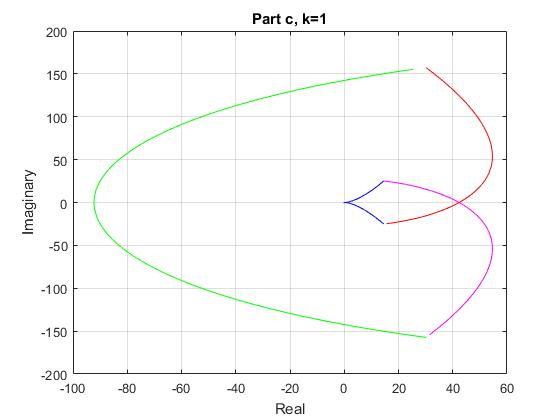
\includegraphics[scale=0.7]{Delay_Part_C_k1.jpg}}
	\subfigure[]{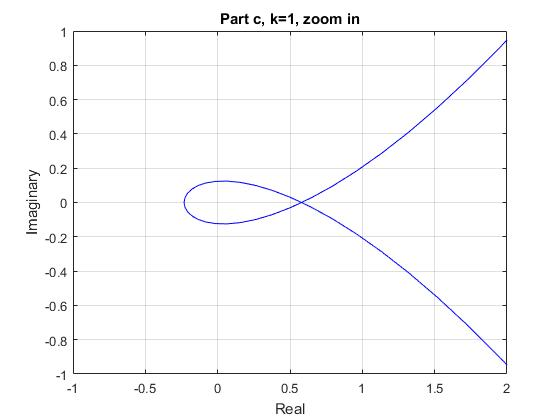
\includegraphics[scale=0.7]{Delay_Part_C_k1_zoom.jpg}}
	\caption{a)k=1; b) k=1, Zoom in}
\end{figure}

Looking at Fig.1.1b (the zoom in), we can see that the curve makes a loop in the clockwise direction around the origin. Therefore we can conclude that no eigenvalue, which are the solutions of our characteristic polynomial, lies inside the rectangle. So, for the case $k$=1, the DDE system is stable.\\

Now, for the case $k$=4 we get

\begin{figure}[H]
	\subfigure[]{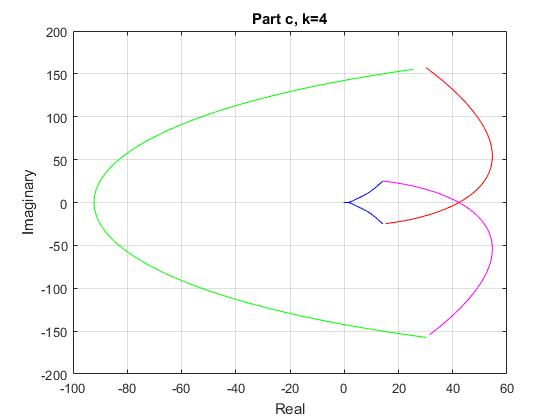
\includegraphics[scale=0.75]{Delay_Part_C_k4.jpg}}
	\subfigure[]{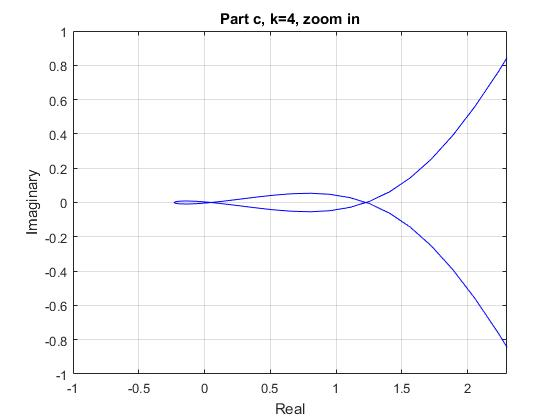
\includegraphics[scale=0.75]{Delay_Part_C_k4_zoom.jpg}}
	\caption{a)k=4; b) k=4, Zoom in}
\end{figure}

Looking at Fig.1.2b (the zoom in), we can see that the curve makes 1 loop in the counterclockwise direction around the origin. Therefore we can conclude that 1 eigenvalue lies inside the rectangle. So, for the case $k$=4, the DDE system is unstable.

\section{Part c - Extra Credit}
We use Matlab $dde23$ to simulate both of these cases and we get
\begin{figure}[H]
	\subfigure[]{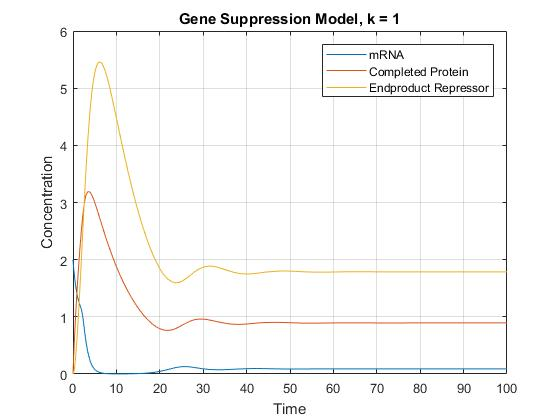
\includegraphics[scale=0.7]{Delay_k1.jpg}}
	\subfigure[]{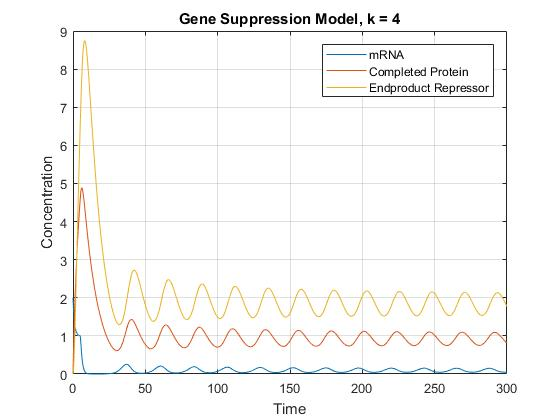
\includegraphics[scale=0.7]{Delay_k4.jpg}}
	\caption{a)k=1; b) k=4}
\end{figure}

Therefore we can conclude that the dynamics of the system depends on the delay $k$. When $k$=1, the soltution monotonically approaches the equilibrium found in Part b.\\
Whereas, for $k$=4, the solution oscillates around the equilibrium.
\section{Part d}
To find where the Hopf bifurcation occurs, we let $\lambda$=i$\omega$ and we substitute it into our characteristic polynomial found in Part c. In order to later use MatLab $\textit{fsolve}$ to solve the system, let's rewrite the polynomial as follows
$$
0.05e^{k\lambda} + 0.65\lambda e^{k\lambda} + 1.6\lambda^{2}e^{k\lambda} + \lambda^{3}e^{k\lambda} + 0.1821 = 0.
$$
Using Euler's formula, we can re-write the polynomyal and split it into real and imaginary parts.\\
So, for the real part we have
$$
0.05cos(k\omega) - 0.65\omega sin(k\omega) - 1.6\omega^{2}cos(k\omega) + \omega^{3}sin(k\omega) + 0.1821 = 0,
$$
whereas for the imaginary part we have
$$
0.05sin(k\omega) + 0.65\omega cos(k\omega) - 1.6\omega^{2}sin(k\omega) - \omega^{3}cos(k\omega) = 0.
$$
So now we can use MatLab $fsolve$ and get the values of $k$ and $\omega$.
And we find
$$
k = 3.8582, \ \omega=0.2868
$$






\end{document}
